\documentclass[a4paper, 11pt, normalem]{report}

\usepackage{../../../LaTeX-Templates/Notes}
\usepackage{subfiles}
\usepackage{epigraph}
\usetikzlibrary{decorations.pathmorphing}
\usetikzlibrary{arrows.meta}

\tikzset{snake it/.style={decorate,decoration=snake}}


\setlength{\epigraphwidth}{\textwidth}
\titleformat{\part}[display]
{\normalfont\huge\filcenter\bfseries\thispagestyle{epigraph}}
{\partname\ \thepart}
{20pt}
{\Huge}
\titlespacing*{\part}{0pt}{0pt}{40pt}

\title{Atoms, Lasers, and Qubits \vspace{-20pt}}
\author{Dr Weatheril and Prof Adams}
\date{\vspace{-15pt}Michaelmas Term 2019 - Epiphany Term 2020}
\rhead{\hyperlink{page.1}{Contents}}

\begin{document}

\maketitle
%\tableofcontents

\epigraphhead[200]{\hfil
\includegraphics[scale=0.5]{lasers.png}\hfil}
\part{}
\chapter{}
\begin{itemize}
    \item \textbf{Note:} The course will be more reading based than math based. 
Read the references on each summary sheet. 
    \item Need light oscillation, not just amplification.  
    \item 1 in $10^{18}$ atomic clock accuracy.
    \item LD: laser diode
    \item Non-linear crystals allow different wavelengths
    \item Laser transitions based on E group of materials
    \item Learn the unit conversions
    \item Magneto-optical trap to cool atoms
    \item Optical frequency comb $\to$ accurate measurement of wavelength of light 
    \item Sodium atoms in upper atmosphere which we fluoresce for AO
    \item \textbf{LEARN!} Q on paper always - contents of a laser
        \begin{enumerate}
            \item More in excited state than ground
            \item Pump gets energy in
            \item Mirrors to make light bounce back and forward
        \end{enumerate}
\end{itemize}

\section{Introduction to lasers}
Lasers - coherence $\to$ 2 types - longitudinal and transverse
\begin{itemize}
    \item Lasers are highly coherent, both transversely and longitudinally. 
        Longitudinal and temporal coherence is related to linewidth, and will be discussed. 
        Coherence length $l_c$ and coherence time $\tau_c$ are the distance and time over which a coherent wave maintains a specified degree of coherence, i.e. when its phase is predictable. 
\end{itemize}
\begin{multicols}{2}
\begin{figure}[H]
    \centering
    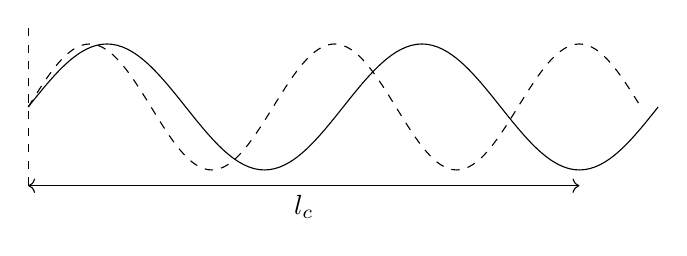
\begin{tikzpicture}
        \draw[dashed] (0,0) -- (0,2);
        \draw[<->] (0,0) -- (7,0) node[anchor=north,midway] {$l_c$};
        \draw (0,1) sin (1,1.8) cos (2,1) sin (3,0.2) cos (4,1) sin (5,1.8) cos (6,1) sin (7,0.2) cos (8,1);
        \draw[dashed] (0,1) sin (0.78,1.8) cos (1.56,1) sin (2.33,0.2) cos (3.11,1) sin (3.89,1.8) cos (4.67,1) sin (5.44,0.2) cos (6.22,1) sin (7,1.8) cos (7.78,1);
    \end{tikzpicture}
\end{figure}
\columnbreak
Coherence length and time:
\begin{align}
    l_c &= \frac{2\pi c}{\delta\om},~~  \tau_c = \frac{2\pi}{\delta\om}
\end{align}
\end{multicols}
\begin{itemize}
    \item Can't have an infinitely narrow spectrum. 
        Monochromaticity - laser has a spectral linewidth $\delta\om$, this is much smaller than the actual carrier/centre frequency. $\delta\om\ll\om_0$ for a laser where $\om_0$ is the centre frequency. 
        From mHz to GHz in range. 
    \item Highly directional beam $\to$ energy contained in one region. 
\end{itemize}
Directionality:
\begin{itemize}
    \item Lasers have highly directional beams that diverge due to diffraction
    \item Beam will be larger
    \item Waist of beam, $2\om_0$.
\end{itemize}
\begin{figure}[H]
    \centering
    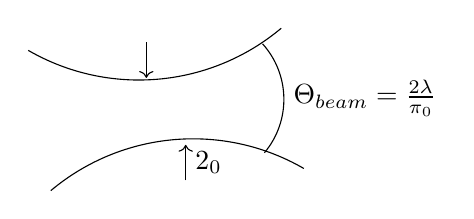
\begin{tikzpicture}
        \draw (0,1) arc (240:310:80pt);
        \draw (3.5,-0.5) arc (60:130:80pt);
        \draw (3,-0.3) arc (-40:42:30pt) node[anchor=west,midway] {$\Theta_{beam} = \frac{2\lambda}{\pi\om_0}$};
        \draw[->] (1.5,1.1) -- (1.5,0.65);
        \draw[->] (2,-0.65) -- (2,-0.2) node[anchor=west,midway] {$2\om_0$};
    \end{tikzpicture}
\end{figure}
\begin{itemize}
    \item All in a very low frequency range $\to$ all energy oscillating in small aarea in small frequency range - useful applications. 
\end{itemize}
Brightness:
\begin{itemize}
    \item Lasers are spectrally bright
    \item Definition of brightness - amount of power in particular area (solid angle) of the beam:
        \begin{equation}
            B_\om = \frac{P}{A\Delta\Om\Delta\om},
        \end{equation}
        where $A$ is the area, $\Delta\Om$ is the solid angle, and $\Delta\om$ is the linewidth. 
\end{itemize}
Electromagnetic Field Modes - not examinable:
\begin{itemize}
    \item 1st Chapter of 'Laser Physics' book
    \item Planck's radiation law
    \item Each unique solution of field is EM mode
    \item $L^3$ factored out when divided by volume
    \item Modes exist with or without energy
\end{itemize}


\chapter{Einstein's rate equations}
A laser requirs amplification due to stimulated emission of radiation. 
\begin{multicols}{2}
\begin{figure}[H]
    \centering
    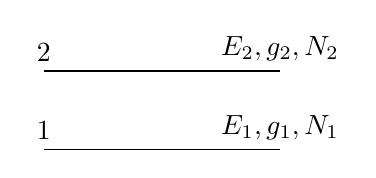
\begin{tikzpicture}
        \draw (0,1) node[anchor=south] {2} -- (3,1) node[anchor=south] {$E_2,g_2,N_2$};
        \draw (0,0) node[anchor=south] {1} -- (3,0) node[anchor=south] {$E_1,g_1,N_1$};
    \end{tikzpicture}
\end{figure}
\begin{align}
    E_2 - E_1 = \hbar\om_{12}
\end{align}
\end{multicols}
\begin{enumerate}
    \item Spontaneous emission: Atom in some excited state, until some time later where it spontaneously decays into a lower state, with a photon emitted with energy shown in Eq (2.1). 
        Rates: $A_{21}$ per $N_i$ atoms, or $A_{21}N_2$ per $m^3$.
        \begin{figure}[H]
            \centering
            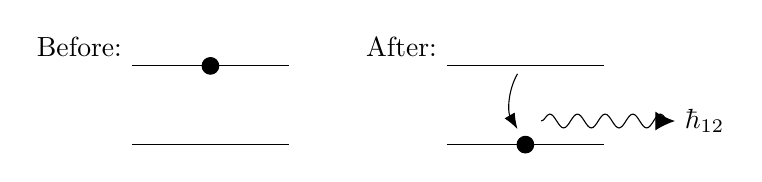
\begin{tikzpicture}
                \draw (0,1) node[anchor=south east] {Before:} -- (2,1);
                \draw[fill] (1,1) circle (3pt);
                \draw (0,0) -- (2,0);

                \draw (4,1) node[anchor=south east] {After:} -- (6,1);
                \draw (4,0) -- (6,0);
                \draw[fill] (5,0) circle (3pt);
                \draw[-{Latex[length=2mm,width=1.5mm]}] (4.9,0.9) arc (150:210:20pt);
                \draw[-{Latex[length=2.5mm,width=2.4mm]},snake it] (5.2,0.3) -- (6.9,0.3) node[anchor=west] {$\hbar\om_{12}$};
            \end{tikzpicture}
        \end{figure}
    \item Absorption: Excite into excited state using energy of photon. 
        Rates: $B_{12}\rho(\om_{12})$, $B_{12}\rho(\om_{12})N_2$.
        \begin{figure}[H]
            \centering
            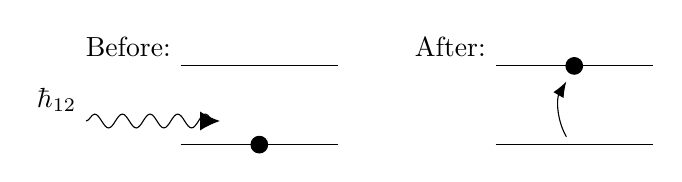
\begin{tikzpicture}
                \draw (0,1) node[anchor=south east] {Before:} -- (2,1);
                \draw[fill] (1,0) circle (3pt);
                \draw (0,0) -- (2,0);    
                \draw[-{Latex[length=2.5mm,width=2.4mm]},snake it] (-1.2,0.3) node[anchor=south east] {$\hbar\om_{12}$} -- (0.5,0.3);

                \draw (4,1) node[anchor=south east] {After:} -- (6,1);
                \draw (4,0) -- (6,0);
                \draw[fill] (5,1) circle (3pt);
                \draw[-{Latex[length=2mm,width=1.5mm]}] (4.9,0.1) arc (210:150:20pt);
            \end{tikzpicture}
        \end{figure}
    \item Stimulated emission: At the initial time we have an atom in an excited state which we then apply a radiated field (photon) to. Later, the atom will decay into a lower state and there will be two outgoing photons - they have been emitted into the same mode.
        Rates: $B_{21}\rho(\om_{12})$, $B_{21}\rho(\om_{12})N_2$. Note: 
        \begin{itemize}
            \item Here, $\rho(\om_{12})$ is the spectral energy density - the energy density, per unit angular frequency range at $\om$, with units of $J\,m^{-3}\,s$.
            \item Generally, the light being used here is broad-band.
        \end{itemize}
        \begin{figure}[H]
            \centering
            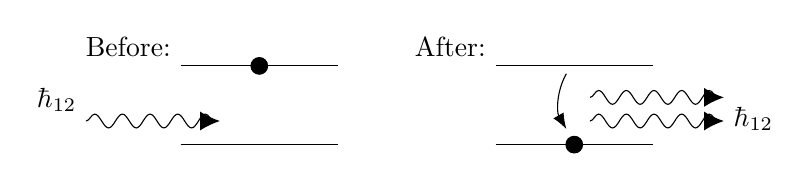
\begin{tikzpicture}
                \draw (0,1) node[anchor=south east] {Before:} -- (2,1);
                \draw[fill] (1,1) circle (3pt);
                \draw (0,0) -- (2,0);    
                \draw[-{Latex[length=2.5mm,width=2.4mm]},snake it] (-1.2,0.3) node[anchor=south east] {$\hbar\om_{12}$} -- (0.5,0.3);
                
                \draw (4,1) node[anchor=south east] {After:} -- (6,1);
                \draw (4,0) -- (6,0);
                \draw[fill] (5,0) circle (3pt);
                \draw[-{Latex[length=2mm,width=1.5mm]}] (4.9,0.9) arc (150:210:20pt);
                \draw[-{Latex[length=2.5mm,width=2.4mm]},snake it] (5.2,0.3) -- (6.9,0.3);
                \draw[-{Latex[length=2.5mm,width=2.4mm]},snake it] (5.2,0.6) -- (6.9,0.6) node[anchor=north west] {$\hbar\om_{12}$};
            \end{tikzpicture}
        \end{figure}
\end{enumerate}

\section{Apply the 3 processess}
\textit{Doodle going through $A_{21}$ to $B_{12}$ to $B_{21}$.}
\begin{figure}[H]
    \centering
    \begin{tikzpicture}
        \draw (0.5,2) node[anchor=south east] {2} -- (7.5,2) node[anchor=south west] {$E_2$};
        \draw (0.5,0) node[anchor=north east] {1} -- (7.5,0) node[anchor=north west] {$E_1$};
        \draw[-{Latex[length=2mm,width=1.5mm]}] (2,2) -- (2,0) node[anchor=east,midway] {$A_{21}$};
        \draw[-{Latex[length=2mm,width=1.5mm]}] (4,0) -- (4,2) node[anchor=east,midway] {$B_{12}\rho(\om_{12})$};
        \draw[-{Latex[length=2mm,width=1.5mm]}] (6,2) -- (6,0) node[anchor=east,midway] {$B_{21}\rho(\om_{12})$};
    \end{tikzpicture}
\end{figure}
Conservation of atom number:
\begin{align}
    \frac{dN_2}{dt} &= -\frac{dN_1}{dt} \\
    N_1 + N_2 &= N = \text{const} \\
    N_1B_{12}\rho(\om_{12}) &= N_2A_{21} + N_2B_{21}\rho(\om_{12})
\end{align}
Rearrange for the spectral energy density:
\begin{align}
    \rho(\om_{12}) &= \frac{N_2A_{21}}{N_1B_{12}-N_2B_{21}} = \frac{\frac{A_{21}}{B_{21}}}{\frac{N_1}{N_2}\frac{B_{12}}{B_{21}} - 1}
\end{align}
Substitute using Boltzmann Law:
\begin{align}
    \frac{N_2}{N_1} &= \frac{g_2}{g_1}\exp\left(-\frac{\hbar\om_{12}}{k_BT}\right) \\
    \implies \rho(\om_{12}) &= \frac{\frac{A_{21}}{B_{21}}}{\frac{g_1}{g_2}\frac{B_{12}}{B_{21}}\exp\left(\frac{\hbar\om_{12}}{k_BT}\right) - 1}
\end{align}
Now look at Planck's Law:
\begin{align}
    \rho(\om) &= \frac{\hbar\om^3}{\pi^2c^3} \frac{1}{\exp\left(\frac{\hbar\om}{k_BT}\right) - 1}
\end{align}
Einstein realised there must be an extra condition to switch between these two forms.
This reveals:
\begin{align}
    g_1B_{12} &= g_2B_{21} \\
    A_{21} &= \frac{\hbar\om_{12}^3}{\pi^2c^3}B_{21}
\end{align}
Notes:
\begin{itemize}
    \item Effectively only 1 coefficient as if we know A, we know B. 
    \item $A_{21}$ is the radiative decay rate,
        \begin{equation}
            A_{21} = \frac{1}{\tau_2}
        \end{equation}
    \item B has units $m^3\,J^{-1}\,s^{-2}$.
    \item A and B are constants for a particular atom.
    \item From the $\om^3$ term, we can see that an infrared transition may decay very fast, but a microwave transition may decay very slow. 
    \item Ratio of $A/B \propto \om^3$ - lasers at high requency harder to achieve.
    \item The principle of detailed balance states that \textbf{\unl{in equilibrium}, the total number of particles entering a quantum state by a partucular rate per unit time is the same as the number leaving by the same rate.}
\end{itemize}

\section{Steady State Solution}
For simplicity, we will assume that $g_1=g_2$ such that the B coefficients are the same. 
\begin{align}
    N_1B_{12}\rho(\om_{12}) &= N_2A_{21} + N_2B_{12}\rho(\om_{12}) \\
    N_1 &= N - N_2
\end{align}
Now we can rearrange to eliminate $N_1$.
\begin{align}
    \frac{N_2}{N} &= \frac{B_{12}\rho(\om_{12})}{A_{21}+2B_{12}\rho(\om_{12})}
\end{align}
Now consider the form of the above as the spectral energy density tends to infinity. 
What we see  is that $N_2 \to \frac{N}{2}$.
This tells us that for at least a two-level atom we cannot get population inversion, which is required for lasers, i.e. steady state inversion impossible.

\section{Number of photons per mode}
$\bar{n}$ can be thought of as the mean number of photons per mode, and $g(\om)\,d\om$ as the mode density. 
\begin{align}
    \rho(\om)\,d\om &= \bar{n} \times g(\om)\,d\om \times \hbar\om
\end{align}
Standard result:
\begin{align}
    g(\om)\,d\om &= \frac{\om^2}{\pi^2c^3}\,d\om \\
    \implies \bar{n} &= \frac{\rho(\om)}{\hbar\om g(\om)} = \frac{\pi^2c^3}{\hbar\om^3}\rho(\om)\\
    \bar{n} = \frac{B_{21}\rho(\om)}{A_{21}} = \frac{\text{rate of stimulated emission}}{\text{rate of spontaneous emission}}
\end{align}
It follows that:
\begin{itemize}
    \item $\bar{n}>1$ - stimulated emission dominates $\implies$ LASERS
    \item $\bar{n}<1$ - spontaneous emission dominates $\implies$ classical light source
\end{itemize}
For a black body:
\begin{align}
    \bar{n} &= \frac{1}{\exp\left(\frac{\hbar\om_{12}}{k_BT}\right) -1} = \frac{B_{12}\rho(\om)}{A_{21}}
\end{align}
These rates are equal when
\begin{align}
    \frac{\hbar\om_{12}}{k_BT} &= \ln(2)
\end{align}
For $\lambda=500\,nm$, $T= 41400\,K$. So for most black bodies, stimulated emission is negligible.

\chapter{Linewidths and Lineshapes}
2 types of broadening:
\begin{itemize}
    \item Homogeneous - all atoms in sample affected the same
    \item Inhomogeneous - atoms in sample affected differently
\end{itemize}

\section{Homogeneous Broadening}
Every atom/molecule exhibits this type of broadening to varying magnitudes.\\
\textbf{Radiative (natural) broadening:}
\begin{itemize}
    \item Consider some excited state population (\textit{doodle}), $N_2$. $e^{-\Gamma_Ht}$
        Leads to some spread in maximum, \textit{doodle}.
        \begin{equation}
            FWHM = \Gamma_H
        \end{equation}
        This broadening follows from the Heisenberg uncertainty principle: Finite lifetime $\implies$ spread in energy, $\Delta E\Delta t \approx \hbar/2$, then a spread in energy $\implies$ a spread in frequency,
        \begin{equation}
            \Delta E = \hbar\Delta\om \implies \Delta\om = \frac{1}{\tau_2} = A_{21} = \Gamma_H
        \end{equation}
        This is only for a 2 level atom.
        \begin{figure}[H]
            \centering 
            \begin{tikzpicture}
                \draw[->] (0,0) -- (0,2) node[anchor=east] {$N_2$};
                \draw[->] (0,0) -- (3,0) node[anchor=west] {$t$};
                \draw (0.2,2) .. controls (0.5,1) and (1.5,0.3) .. (3,0.2) node[anchor=south west] {$e^{-\Gamma_Ht}$};

                \draw[->] (5,0) -- (9,0) node[anchor=west] {$\om$}; 
                \draw (7,-0.1) node[anchor=north] {$\om_{12}$} -- (7,0.1);
                \draw (5.1,0.1) cos (6.7,1.7) sin (7,2) cos (7.3,1.7) sin (8.9,0.1);
                \draw[<->] (6.3,1) -- (7.7,1) node[anchor=south west] {FWHH $= \Gamma_H$};
            \end{tikzpicture}
        \end{figure}
    \item Define the normalised lineshape function:
        \begin{align}
            L_H(\om) &= \frac{\Gamma_H/2\pi}{(\om-\om_{12})^2+\frac{\Gamma_H^2}{4}} \\
            \ofnt &L_H(\om)\;d\om = 1
        \end{align}
    \item For multiple decay paths: 
        \begin{multicols}{2}
        \begin{figure}[H]
            \centering
            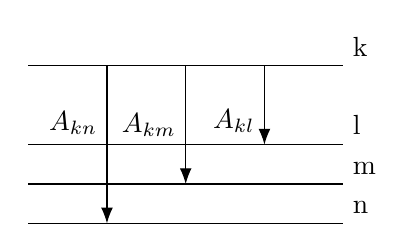
\begin{tikzpicture}
                \draw (0,2) -- (4,2) node[anchor=south west] {k};
                \draw (0,1) -- (4,1) node[anchor=south west] {l};
                \draw (0,0.5) -- (4,0.5) node[anchor=south west] {m};
                \draw (0,0) -- (4,0) node[anchor=south west] {n};

                \draw[-{Latex[length=2mm,width=1.5mm]}] (1,2) -- (1,0) node[anchor= south east,midway] {$A_{kn}$};
                \draw[-{Latex[length=2mm,width=1.5mm]}] (2,2) -- (2,0.5) node[anchor=east,midway] {$A_{km}$};
                \draw[-{Latex[length=2mm,width=1.5mm]}] (3,2) -- (3,1) node[anchor=north east,midway,yshift=2pt] {$A_{kl}$};
            \end{tikzpicture}
        \end{figure}
        For level k
        \begin{align}
            \frac{dN_k}{dt} &= -N_kA_{kl} - N_kA_{km} - N_kA_{kn} \\
            \tau_k &= \frac{1}{\sum A_{ki}} = \frac{1}{\Gamma_H}
        \end{align}
        \end{multicols}
    \item When both levels decay:
        \begin{figure}[H]
            \centering
            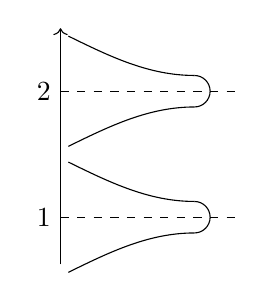
\begin{tikzpicture}
                \draw[->] (0,0) -- (0,3);
                \draw (0.1,2.9) sin (1.7,2.4);
                \draw (1.7,2.4) arc (90:-90:0.2cm);
                \draw (1.7,2) cos (0.1,1.5);
                
                \draw (0.1,1.3) sin (1.7,0.8);
                \draw (1.7,0.8) arc (90:-90:0.2cm);
                \draw (1.7,0.4) cos (0.1,-0.1);

                \draw[dashed] (0,2.2) node[anchor=east] {2} -- (2.3,2.2);
                \draw[dashed] (0,0.6) node[anchor=east] {1} -- (2.3,0.6);
            \end{tikzpicture}
        \end{figure}
        \begin{align}
            \Gamma_2 &= \sum A_{2i} = \frac{1}{\tau_2} \\
            \Gamma_1 &= \sum A_{1i} = \frac{1}{\tau_1} \\
            \Gamma_{21} &= \Gamma_2 + \Gamma_1
        \end{align}
        $\Gamma_{21}$ is the emission linewidth. 
\end{itemize}
\begin{example}[Argon ion laser]
    \begin{figure}[H]
        \centering
        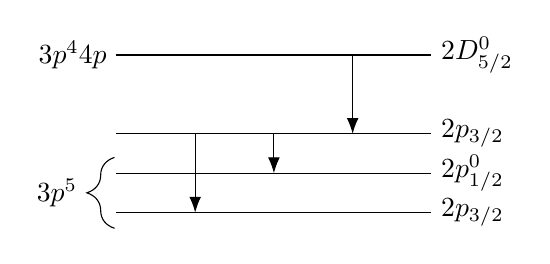
\begin{tikzpicture}
            \draw (0,2) node[anchor=east] {$3p^44p$} -- (4,2) node[anchor=west] {$2D_{5/2}^0$};
            \draw (0,1) -- (4,1) node[anchor=west] {$2p_{3/2}$};
            \draw (0,0.5) -- (4,0.5) node[anchor=west] {$2p_{1/2}^0$};
            \draw (0,0) -- (4,0) node[anchor=west] {$2p_{3/2}$};

            \draw[-{Latex[length=2mm,width=1.5mm]}] (3,2) -- (3,1);
            \draw[-{Latex[length=2mm,width=1.5mm]}] (2,1) -- (2,0.5);
            \draw[-{Latex[length=2mm,width=1.5mm]}] (1,1) -- (1,0);

            \draw[decorate,decoration={brace,amplitude=10pt},xshift=5pt] (-0.2,-0.2) -- (-0.2,0.7) node[midway,anchor=east,xshift=-10pt] {$3p^5$}; 
        \end{tikzpicture}
    \end{figure}
    $\lambda = 488\,nm$, $A= 7.8\times10^7\;s^{-1}$, $1:\,73,1\;nm;~ A=4.5\times10^8\;s^{-1}$, $2:\,72.3\;nm;~ A=23\times10^8\;s^{-1}$.\\
    Emission linewidth:
    \begin{align}
        \sum A &= 2.8\times10^9 = (2\pi)450\;MHz
    \end{align}
\end{example}
\textbf{Collisional/pressure broadening:}
\begin{itemize}
    \item Collisions between atoms - de-excite the atoms $\to$ reduce excited state lifetime $\to$ broader transition
    \item Depends on pressure - important for gas lasers
\end{itemize}
\textbf{Phonon broadening:}
\begin{itemize}
    \item \textit{doodle of standard 1,2 transition for bare atom/ion}. In a crystal, two distinct groups of energy levels packed together, quantised vibrational modes $\implies$ phonons. 
    \item Occurs in solid state lasers, and is temperature tempendent
    \item Dominant broadening at room temperature
\end{itemize}

\section{Inhomogeneous Broadening}
\textbf{Doppler Broadening:}
\begin{itemize}
    \item Arises due to motion of atoms - when a moving atom emits, there is a Doppler shift dependent on the component of velocity along the direction of the emitted photon.
        \begin{align}
            \om &= \om_{12}\left(1 \pm \frac{v_z}{c}\right)
        \end{align} 
        $\pm$ for blue/red shift - blue as velocity towards observer, red away. 
    \item Broadening arises due to Maxwell-Boltzmann distribution of velocities,
        \begin{align}
            P(v_z)\,dv_z &= \left(\frac{M}{2\pi k_BT}\right)^{1/2} \exp\left(-\frac{Mv_z^2}{2k_BT}\right)\;dv_z
        \end{align}
        Use correspondence between $v_z$ and $\om$ to get
        \begin{figure}[H]
            \centering
            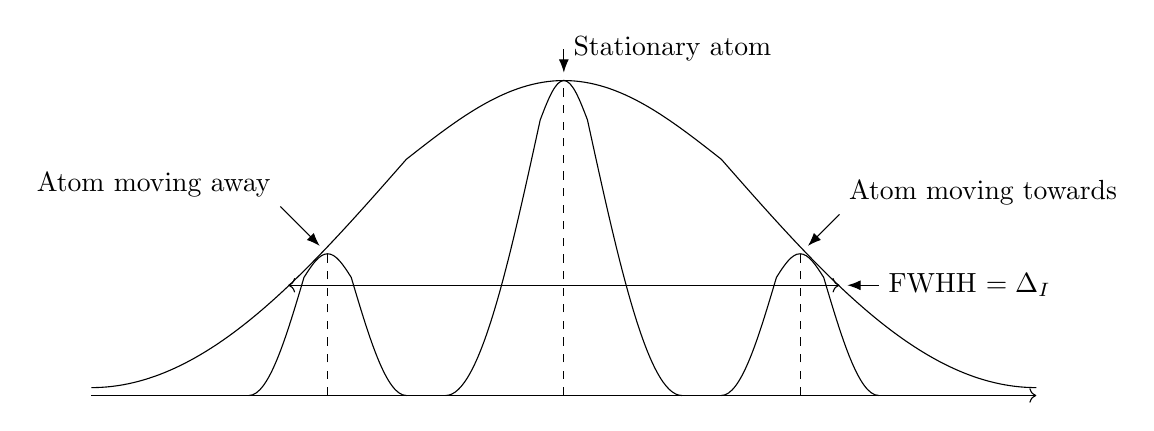
\begin{tikzpicture}
                \draw[->] (0,0) -- (12,0);
                \draw (0,0.1) cos (4,3) sin (6,4) cos (8,3) sin (12,0.1);
                \draw (2,0) cos (2.7,1.5) sin (3,1.8) cos (3.3,1.5) sin (4,0);
                \draw (4.5,0) cos (5.7,3.5) sin (6,4) cos (6.3,3.5) sin (7.5,0);
                \draw (8,0) cos (8.7,1.5) sin (9,1.8) cos (9.3,1.5) sin (10,0);

                \draw[dashed] (3,0) -- (3,1.8);
                \draw[dashed] (6,0) -- (6,4);
                \draw[dashed] (9,0) -- (9,1.8);

                \draw[<->] (2.5,1.4) -- (9.5,1.4);
                \draw[-Latex] (10,1.4) node[anchor=west] {FWHH $= \Delta\om_I$} -- (9.6,1.4);
                \draw[-Latex] (9.5,2.3) node[anchor=south west] {Atom moving towards} -- (9.1,1.9);
                \draw[-Latex] (2.4,2.4) node[anchor=south east] {Atom moving away} -- (2.9,1.9);
                \draw[-Latex] (6,4.4) node[anchor=west] {Stationary atom} -- (6,4.1);
            \end{tikzpicture}
        \end{figure}
        \begin{align}
            P(\om)\,d\om &= \frac{c}{\om_{12}}\left(\frac{M}{2\pi k_BT}\right)^{1/2}\exp\left[-\frac{Mc^2}{2k_B T}\frac{(\om-\om_{12})^2}{\om_{12}^2}\right]
        \end{align}
    \item For Doppler broadening, 
        \begin{align}
            \Delta\om_I &= \frac{2\om_{12}}{c}\left(\frac{2k_BT}{M}\ln2\right)^{1/2} \\
                        &= 7.16\times10^{-7}\om_{12}\left(\frac{T}{M_A}\right)^{1/2}
        \end{align}
        $\Delta\om_I$ is known as the Doppler width, $M_A$ is using the mass in atomic units instead of kg as used so far for $M$.
\end{itemize}
\begin{example}[Argon ion laser 2]
$M_A = 40$, $\lambda=488\,nm$, Discharge temperature $\approx 1200^\circ C$.
\begin{align}
    \Delta\om_I &= (2\pi) 2.7\,GHz
\end{align}
This is many times larger than the natural broadening. 
\end{example}
\textbf{Amorphous crystal broadening:}
\begin{itemize}
    \item Occurs in glass materials
    \item Inhomogeneities are Gaussian (normal), the emission is also Gaussian
\end{itemize}

\chapter{}
\begin{example}
\begin{figure}[H]
    \centering
    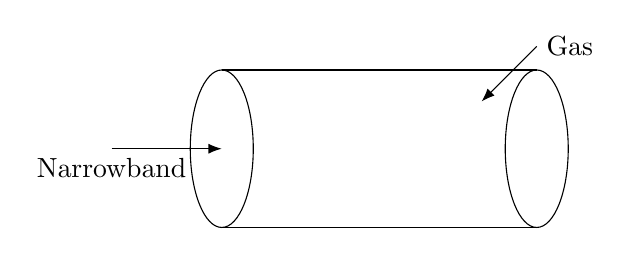
\begin{tikzpicture}
        \draw (0,0) ellipse (0.4cm and 1cm);
        \draw (0,1) -- (4,1);
        \draw (0,-1) -- (4,-1);
        \draw (4,0) ellipse (0.4cm and 1cm);
        \draw[-Latex] (4,1.3) node[anchor=west] {Gas} -- (3.3,0.6);

        \draw[-Latex] (-1.4,0) node[anchor=north] {Narrowband} -- (0,0);
    \end{tikzpicture}
\end{figure}
If the light beam is resonant with the atoms in the gas, we would expect some interaction. 
But how is the medium excited?
It depends on the broadening. 
\begin{enumerate}
    \item Homogeneous broadening (Lorentzian):
        \begin{figure}[H]
            \centering
            \begin{tikzpicture}
                \draw[->] (-3,0) -- (3,0) node[anchor=north] {$\om$};
                \draw[->] (0,0) node[anchor=north] {$\om_{12}$} -- (0,4) node[anchor=east] {$N_1$};
                \draw (-2.8,0.1) cos (-0.4,3.2) sin (0,3.8) cos (0.4,3.2) sin (2.8,0.1);

                \draw[-Latex] (3,2) -- (4,2);

                \draw[->] (4,2.5) -- (10,2.5) node[anchor=north] {$\om$};
                \draw[->] (7,2.5) node[anchor=north] {$\om_{12}$} -- (7,4.5) node[anchor=east] {$N_2$};
                \draw[dashed] (4.2,2.6) cos (6,3.5) sin (7,3.8) cos (8,3.5) sin (9.8,2.6);

                \draw[->] (4,-1) -- (10,-1) node[anchor=north] {$\om$};
                \draw[->] (7,-1) node[anchor=north] {$\om_{12}$} -- (7,2) node[anchor=east] {$N_1$};
                \draw (4.2,-0.8) cos (6.4,1.2) sin (7,1.8) cos (7.6,1.2) sin (9.8,-0.8);
                \draw[dashed] (4.2,-0.9) cos (6.4,0.8) sin (7,1.4) cos (7.6,0.8) sin (9.8,-0.9);
            \end{tikzpicture}
        \end{figure}
        Turn on radiation within natural linewidth. 
        All of these distributions will be the same - all atoms are affected equally, and the population of $N_1$ is reduced slightly as it moves into $N_2$.
    \item Inhomogeneous broadening (Gaussian): 
        \begin{figure}[H]
            \centering
            \begin{tikzpicture}
                \draw[->] (-3,0) -- (3,0) node[anchor=north] {$\om$};
                \draw[->] (0,0) node[anchor=north] {$\om_{12}$} -- (0,3) node[anchor=east] {$N_1$};
                \draw (-2.8,0.1) cos (-1,2) sin (0,2.8) cos (1,2) sin (2.8,0.1);
                \draw[fill] (0.75,0) rectangle (1.25,0.6);

                \draw[-Latex] (3,1.5) -- (4,1.5);

                \draw[->] (4,2.5) -- (10,2.5) node[anchor=north] {$\om$};
                \draw[->] (7,2.5) node[anchor=north] {$\om_{12}$} -- (7,3.5) node[anchor=east] {$N_2$};
                \draw[dashed] (7.5,2.5) cos (7.9,3) sin (8,3.2) cos (8.1,3) sin (8.5,2.5);

                \draw[->] (4,-1) -- (10,-1) node[anchor=north] {$\om$};
                \draw[->] (7,-1) node[anchor=north] {$\om_{12}$} -- (7,2) node[anchor=east] {$N_1$};
                \draw (4.1,-0.9) cos (6,0.8) sin (7,1.5) cos (7.5,1) sin (8,-0.2) cos (8.5,0.2) sin (9.9,-0.9);
            \end{tikzpicture}
        \end{figure}
        Distributions are now very different - atoms are affected differently, and only a subset of the atoms interact.
        For example, with Doppler broadening, only particles with a specific velocity would be excited strongly by the light beam. 
        The width of the N2 Gaussian is determined by natural broadening. 
\end{enumerate}
\end{example}
Reminder:
\begin{align}
    A_{21}N_2 &\equiv \text{rate of spontaneous emission per }m^3 \\
    B_{12}\rho(\om_{12})N_1 &\equiv \text{rate of absorption per }m^3 \\
    B_{21}\rho(\om_{12})N_2 &\equiv \text{rate of stimulated emission per }m^3
\end{align}
\section{Homogeneous broadening}
All atoms are affected the same $\implies$ simply define a new constant:
\begin{align}
    a_{21}(\om) &= A_{21}L_H(\om) & b_{12}(\om) &= B_{12}L_H(\om) & b_{21}(\om) &= B_{21}L_H(\om)
\end{align}
Then if we wanted to know the rate of emission now:
\begin{align}
    a_{21}(\om)\,d\om &= \text{rate of emission in range $\om\to\om+d\om$ per atom} 
\end{align}
We have to multiply by the $d\om$ because $L_H(\om)$ has units $\frac{1}{\om}$.
Integrating recovers the result,
\begin{align}
    \int L_H(\om)\,d\om &= 1
\end{align}
Inhomogeneous broadening is more difficult. 
We want to do this, but we can use the results from homogeneous broadening in certain circumstances, i.e. for narrowband light and $\Gamma_H \ll \Delta\om_I$.

\begin{figure}[H]
    \centering
    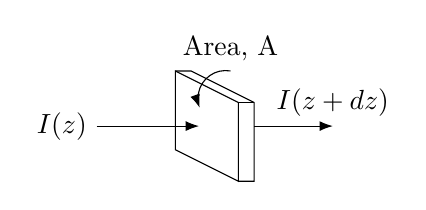
\begin{tikzpicture}
        \draw (0,0) -- (0.8,-0.4) -- (0.8,0.6) -- (0,1) -- cycle;
        \draw (0.8,-0.4) -- (1,-0.4) -- (1,0.6) -- (0.2,1) -- (0,1);
        \draw (1,0.6) -- (0.8,0.6);

        \draw[-Latex] (-1,0.3) node[anchor=east] {$I(z)$} -- (0.3,0.3);
        \draw[-Latex] (1,0.3) -- (2,0.3) node[anchor=south] {$I(z+dz)$};
        \draw[-Latex] (0.7,1) node[anchor=south] {Area, A} arc (80:200:10pt);
    \end{tikzpicture}
\end{figure}
Consider a \unl{weak} narrowband beam of light, frequency $\om$ and bandwidth $d\om$. \\
Assume:
\begin{itemize}
    \item No spontaneous emission
    \item Homogeneous broadening
    \item Steady state
\end{itemize}
Find change in power of beam.
\begin{align}
    \left(I(z+dz) - I(z)\right)A &= \left[N_2B_{21}L_H(\om)\rho(\om_{12})\,d\om - N_1B_{12}L_H(\om)\rho(\om_{12})\,d\om\right]\times\hbar\om\times A\,dz
\end{align}
The term inside the square brackets above is the net rate of photons added to the field ($m^{-3}$).\\
For a beam, the intensity is described as
\begin{align}
    I(z) &= c\rho(\om)\;d\om 
\end{align}
Substitute this into Eq (4.7) and rearrange, also using the expressions for A and B coefficients found in lecture 2: 
\begin{align}
    \frac{1}{I}\frac{dI}{dz} &= \frac{\hbar\om}{c}L_H(\om)\left[N_2B_{21} - N_1B_{12}\right] \\
                             &= \frac{\pi^2c^2}{\om^2_{12}}A_{21}L_H(\om)\left[N_2 - \frac{g_2}{g_1}N_1\right]
\end{align}
This uses the assumption that we are close to resonance.\\
The prefactor can be defined as the optical gain cross section,
\begin{align}
    \sigma(\om) &= \frac{\pi^2c^2}{\om_{12}^2}A_{21}L_H(\om).
\end{align}
Solve equation:
\begin{align}
    I(z) &= I(0)\exp\left[\sigma(\om)\times\left(N_2-\frac{g_2}{g_1}N_1\right)z\right]
\end{align}
There are two cases:
\begin{enumerate}
    \item Absorption:
        \begin{align}
            N_2 &< \frac{g_2}{g_1}N_1 \\
            \implies I(z) &= I(0)e^{-\kappa(\om)z},~ \kappa(\om) = \sigma(\om)\left(\frac{g_2}{g_1}N_1 - N_2\right)  
        \end{align}
        $\kappa$ is the absorption coefficient. 
        \begin{figure}[H]
            \centering
            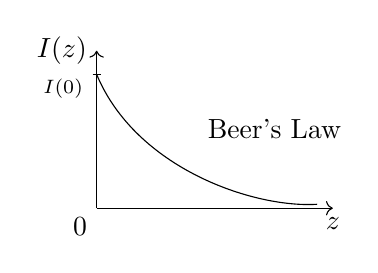
\begin{tikzpicture}
                \draw[->] (0,0) -- (0,2) node[anchor=east] {$I(z)$};
                \draw[->] (0,0) node[anchor=north east] {0} -- (3,0) node[anchor=north] {$z$};
                \draw (0,1.7) .. controls (0.5,0.5) and (2,0) .. (2.8,0.05) node[anchor=south west,midway,yshift=10pt] {Beer's Law};
                \draw (-0.05,1.7) node[anchor=east,yshift=-5pt] {\scriptsize $I(0)$} -- (0.05,1.7);
            \end{tikzpicture}
        \end{figure}
    \item Amplification.
        \begin{align}
            N_2 &> \frac{g_2}{g_1}N_1 \\
            I(z) &= I(0)e^{g(\om)z},~ g(\om) = \sigma(\om)\left(N_2-\frac{g_2}{g_1}N_1\right)
        \end{align}
        $g(\om)$ is the gain coefficient, $e^{g(\om)z}$ is the gain. 
        \begin{figure}[H]
            \centering
            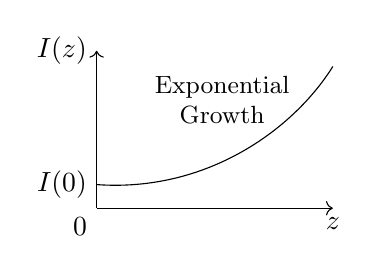
\begin{tikzpicture}
                \draw[->] (0,0) -- (0,2) node[anchor=east] {$I(z)$};
                \draw[->] (0,0) node[anchor=north east] {0} -- (3,0) node[anchor=north] {$z$};
                \draw (0,0.3) node[anchor=east] {$I(0)$} .. controls (1.4,0.2) and (2.5,1) .. (3,1.8) node[anchor=north,xshift=-40pt] {\small \shortstack{Exponential \\ Growth}};
            \end{tikzpicture}
        \end{figure}
\end{enumerate}
The condition for gain is
\begin{equation}
    N_2 > \frac{g_2}{g_1}N_1.
\end{equation}
This is known as \unl{Population Inversion.}
Frequency dependence of the gain:
\begin{align}
    g(\om) &= \sigma(\om)\times N^*, ~ N^* = N_2 - \frac{g_2}{g_1}N_1 \\
           &= \frac{\pi^2c^2}{\om_{12}^2}A_{21}L_H(\om)\times \left[N_2-\frac{g_2}{g_1}N_1\right]
\end{align}
We call $N^*$ the population inversion density. 
\textbf{Note:} Frequency dependence is in the optical gain cross section via $L(\om)$. 
$\sigma(\om)$ is determined by the atom, we cannot control it. 
Broadening spreads gain over a range of frequencies. 

\chapter{}
\begin{figure}[H]
    \centering
    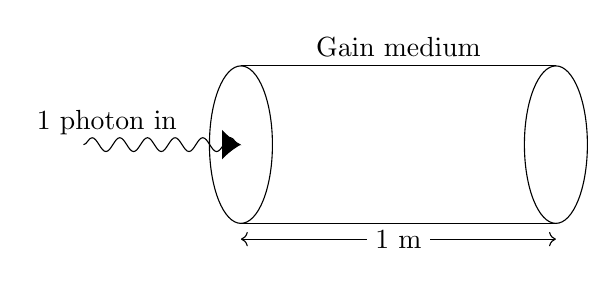
\begin{tikzpicture}
        \draw[-{Latex[length=2.4mm,width=3.8mm]},snake it] (-1,0) -- (1,0) node[anchor=south,midway,xshift=-20pt] {1 photon in};
        \draw (5,0) ellipse (0.4cm and 1cm);
        \draw (1,0) ellipse (0.4cm and 1cm);
        \draw (1,1) -- (5,1) node[anchor=south,midway] {Gain medium};
        \draw (1,-1) -- (5,-1);
        \draw[->] (2.6,-1.2) -- (1,-1.2);
        \draw[->] (3.4,-1.2) -- (5,-1.2);
        \draw[white] (2.6,-1.2) -- (3.4,-1.2) node[midway,black] {1 m};
    \end{tikzpicture}
\end{figure}
Imagine we have a sample which is our laser gain sample, and we will send one photon in. 
For most lasers,  the peak gain, $g(\om_{12}) \approx 0.01\;cm^{-1}$.
So one photon in to our 1m long sample, means $e^1 = 2.7$ photons out.
We must add a cavity to recirculate the light, and now using mirrors either side of the gain medium,  we will pass through the gain medium 40 times, $e^{40} \approx 10^{17}$ photons.
\begin{figure}[H]
    \centering
    \begin{tikzpicture}
        \draw (0,3) arc (120:240:40pt);
        \draw (4,3) arc (60:-60:40pt);
        \draw[-{Latex[length=2mm,width=2mm]}] (0.5,1.6) arc (315:60:0.3cm);
        \draw (1,1.25) rectangle (3,2.25);
        \draw[-{Latex[length=2mm,width=2mm]}] (3.5,2.05) arc (135:-120:0.3cm);
    \end{tikzpicture}
\end{figure}

\section{General Cavity Design}
Also distributed loss throughout cavity of $\alpha$ per meter.

\section{Longitudinal Cavity Modes}
The field in ithe cavity forms standing waves, i.e.
\begin{equation}
    n\frac{\lambda_n}{2} = L_c
\end{equation}
$n$ is called the mode order.
Mode separation,
\begin{equation}
    \Delta\nu_{fsr} = \nu_{n+1} - \nu_n = \frac{c}{2L_c}
\end{equation}
This is the \unl{Free Spectral Range.}
\begin{example}[Mode order of 10cm cavity at $\lambda= 500\,nm$]
    \begin{align}
        n &= \frac{2L_c}{\lambda} = 4\times10^5 \\
        \Delta\nu_{fsr} &= \frac{c}{2L_c} = 1.5\;Ghz
    \end{align}
\end{example}

\section{Cavity Losses}
Trace intensity around the cavity:
\begin{align}
    I_0 \implies I_0R_1(1-a)R_2(1-a)e^{-2\alpha L_c}
\end{align}
\begin{multicols}{2}
\begin{itemize}
    \item Pass through the cavity twice, so $(1-a)$ twice. 
    \item $e^{-2\alpha L_c}$ is the distributed loss over length, $2L_c$.
\end{itemize}
\end{multicols}
\begin{equation}
    I_0 \implies I_0R_1R_2(1-a)^2e^{-2\alpha L_c}
\end{equation}
Express as round trip loss,
\begin{align}
    I_0 &\implies I_0e^{-\delta_c} \\
    \delta_c &= \ln\left(\frac{1}{R_1R_2(1-a)^2}\right)+2\alpha L_c \\
    \frac{I_0-I_0e^{-\delta_c}}{I_0} &= 1 - e^{-\delta_c} \approx 1-(1-\delta_c) = \delta_c
\end{align}
This is the \unl{Fractional Round Trip Loss.}

\section{Cavity Lifetime}
The lifetime of a photon in a cavity is a useful concept. 
Define cavity lifetime, $\tau_c$.
\begin{align}
    I(t) &= I_0e^{-t/\tau_c} \\
         &= I_0e^{-N\delta_c} = I_0e^{-t\delta_c/T_{RT}} \\
    \tau_c &= \frac{2L_c}{c\delta_c} = \frac{T_{RT}}{\delta_c}
\end{align}
$T_{RT}$ is called the Round Trip Time.
Cavity has a quality factor, 
\begin{align}
    Q = \frac{\om}{\Delta\om_c} = \om\tau_c
\end{align}
So we can then think of cavities as having a linewidth, $\Delta\om_c = \frac{1}{\tau_c}$.

\section{Threshold Condition}
\begin{align}
    \text{Round Trip Gain}\times\text{Round Trip Loss} = 1
\end{align}
\begin{itemize}
    \item Gain x loss $>1$, intensity grows $\implies$ laser oscillation 
    \item Gain x loss $<1$, intensity decays $\implies$ no laser :(
\end{itemize}
Substitute for gain and loss:
\begin{align}
    e^{2g(\om_{12}L_m}\times e^{-\delta_c} &= 1 \\
    g_{th}(\om_{12}) &= \frac{\delta_c}{2L_m}
\end{align}

\begin{example}[Helium Neon Laser]
    \begin{itemize}
        \item Gain cell length $= L_m = L_c = 50\,cm$.
        \item Two mirrors with $R_1 = 0.998$ and $R_2 = 0.98$.
        \item Distributed losses are $\alpha = 0.02\,m^{-1}$.
        \item $A_{21} = 3.4\times10^6\,s^{-1},~ \lambda = 632.8\,nm$.
        \item Doppler width is dominant as it is a gas (could be pressure broadening, but assume not for this) - $\Delta\om_I = 2\pi\cdot1500\;MHz$.
    \end{itemize}
    So what is the population inversion density, $N^*$, required for laser oscillation?
    \begin{itemize}
        \item Considering round trip losses
        \item Fractional round trip loss
        \item Atomic properties for expression of gain
        \item Only thing left to then find is $N^*$
    \end{itemize}
\end{example}

\chapter{}
\section{Gain Saturation}
\textit{doodle this too - start with two levels, 1 and 2, $S_1$ and $S_2$, $N_i/\tau_i$, $N_2A_{21}$ - rate between states.}
Develop rate equations for $N_1$ and $N_2$.
\begin{align}
    \frac{dN_2}{dt} &= S_2 - \frac{N_2}{\tau_2} \\
    \frac{dN_1}{dt} &= S_1 + N_2A_{21} - \frac{N_1}{\tau_1}
\end{align}
In the steady state, 
\begin{align}
    \frac{dN_2}{dt} &= \frac{dN_1}{dt} = 0 \\
    N_2 &= S_2\tau_2 \\
    N_1 &= S_1\tau_1 + A_{21}\tau_1N_2 \\
        &= S_1\tau_1 + A_{21}\tau_1S_2\tau_2
\end{align}
Population inversion density,
\begin{align}
    N_0^* &= N_2 - \frac{g_2}{g_1}N_1 \\
        &= S_2\tau_2\left(1-\frac{g_2}{g_1}A_{21}\tau_1\right) - \frac{g_2}{g_1}S_1\tau_1
\end{align}
'0' denotes small signal coefficient (in the absence of field).
\textit{doodle neq two level diagram, same one again, now new arrows up and down}
\begin{align}
    N_2\sigma(\om)\frac{I}{\hbar\om} & \frac{g_2}{g_1}N_1\sigma(\om)\frac{I}{\hbar\om}
\end{align}
We have assumed $L(\om) < \Gamma_{21}$.
\begin{align}
    \frac{dN_2}{dt} &= S_2 - \frac{N_2}{\tau_2} - N^*\sigma(\om)\frac{I}{\hbar\om} \\
    \frac{dN_1}{dt} &= S_1 - \frac{N_1}{\tau_1} + N^*\sigma(\om)\frac{I}{\hbar\om} + A_{21}N_2 \\
    N_2 &= S_2\tau_2 - N^*\left(\frac{\sigma I}{\hbar\om}\right)\tau_2 \\
    N_1 &= S_1\tau_1 + N^*\left(\frac{\sigma I}{\hbar\om}\right)\tau_1 + A_{21}\tau_1N_2 \\
    N^* &= \frac{S_2\tau_2\left(1-\frac{g_2}{g_1}A_{21}\tau_1\right) - \frac{g_2}{g_1}S_1\tau_1}{1+\left(\frac{\sigma I}{\hbar\om}\right)\left[\tau_2+\frac{g_2}{g_1}\left(1-A_{21}\tau_2\right)\tau_1\right]}
\end{align}
Numerator is $N_0^*$:
\begin{align}
    N^* &= \frac{N_0^*}{1 + \frac{I}{I_s}}
\end{align}
We can now define Saturation Intensity:
\begin{align}
    I_s(\om) &= \frac{\hbar\om}{\sigma(\om)}\frac{1}{\tau_2+\frac{g_2}{g_1}\tau_1(1-A_{21}\tau_2)}
\end{align}
Gain is saturated too, since
\begin{align}
    g(\om) &= \sigma(\om)N^* = \frac{g_0(\om)}{1 + \frac{I}{I_s(\om)}}
\end{align}
\textbf{Comments:}
\begin{itemize}
    \item At $I = I_s(\om) \to g(\om) = \frac{g_0(\om)}{2}$.
    \item $I_s(\om)$ is frequency dependent through $\sigma(\om)$, so will happen quicker at line centre.
    \item For an efficient laser, expect large population inversion $\implies \tau_2 \gg \tau_1$.
    \item All decays from state 2 into state 1 $\implies A_{21} \approx \frac{1}{\tau_2}$.
\end{itemize}
\begin{align}
    I_s(\om) &= \frac{\hbar\om}{\sigma(\om)\tau_2}
\end{align}
This is usually an excellent approximation.
\begin{example}[Linear Amplifier]
    \textit{doodle I0 in, IL out of parallelogram that is L long}
    \begin{align}
        \frac{dI}{dz} &= g(\om)I = \frac{g_0(\om)I}{1 + \frac{I}{I_s(\om)}}
    \end{align}
    We just integrate this, after length L:
    \begin{align}
        \int_{I(0)}^{I(L)} \frac{1+\frac{I}{I_s(\om)}}{I}\,dI &= \int_0^L g_0(\om)\,dz \\
        \ln\left(\frac{I_L}{I_0}\right) + \frac{I_L-I_0}{I_s(\om)} &= g_0(\om)L
    \end{align}
    \textbf{Two limiting cases:}
    \begin{enumerate}
        \item $I/I_s(\om) \ll 1 \implies$ exponential growth,
            \begin{align}
                I_L &= I_0e^{g_0(\om)L}
            \end{align}
        \item $I/I_s(\om) \gg 1 \implies$ linear growth,
            \begin{align}
                I_L &= I_0  + g_0(\om)I_s(\om)L
            \end{align}
    \end{enumerate}
    \textit{doodle plot of exp growth into linear growth as z increases}
    \begin{figure}[H]
        \centering
        \begin{tikzpicture}
            \draw[->] (0,0) -- (0,2.5);
            \draw[->] (0,0) -- (4,0);
        \end{tikzpicture}
    \end{figure}
\end{example}


\end{document}















